The chapter is devoted to a general description of the operation of individual parts of the application, both from the perspective of the user and the source code.

\section{Graphical user interface}
  The graphical user interface (GUI) is a simple HTML form, available by default in a web browser window after running the application at the local host address on port 8080: 
	\smallbreak
	\href{http://localhost:8080/flowchart/}{localhost:8080/flowchart/}.
	\bigbreak	
  By default, the GUI contains a field with a generated flowchart diagram in the upper part, and a drop-down select menu, which allows the user to select the syntax of both Mermaid and C-based code, a text area for entering the code itself and a button confirming the submission of the selected syntax type and entered code via Rest API. HTTP requests of type GET handled by the Rest controller allowing two optional parameters: syntax type ($type$) -- Mermaid by default, code placed in the text field ($originalCode$) -- by default drawing two simple blocks. Any throwing of an exception by the program is handled by the controller, and then the message contained in it is forwarded to the error screen.
	
\begin{figure}[H]
  \begin{subfigure}{\textwidth}
    \centering
    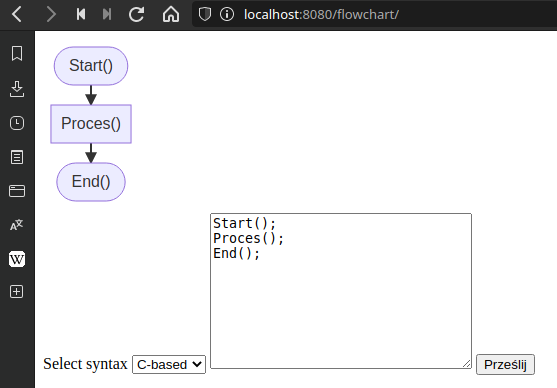
\includegraphics[width=0.8\textwidth]{GUI.png}
  \end{subfigure}\hfill
  \caption{GUI displayed in web browser (Vivaldi 5)}
\end{figure}

Example flowchart available under the URL address: 
	\smallbreak
	\href{http://localhost:8080/flowchart/?type=C\&originalCode=Start();Proces();End();}{http://localhost:8080/flowchart/?type=C\&originalCode=Start();Proces();End();}
	\bigbreak
	
  An additional screen is an HTML page that displays a syntax error message and shows the code fragment where the error occurred.
	
\begin{figure}[H]
  \begin{subfigure}{\textwidth}
  \centering
    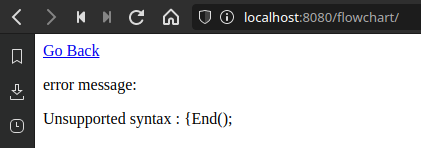
\includegraphics[width=0.8\textwidth]{error-page.png}
  \end{subfigure}\hfill
    \begin{subfigure}[t]{0.44\textwidth}
    \bigbreak
    Generated for the below code:
    \centering
    \begin{minted}[linenos=true]{cpp}    
Start();
Proces();{
End();
    \end{minted}
  \end{subfigure}%
  \caption{Example of a screen displaying syntax error}
\end{figure}


\begin{figure}[H]
	\begin{subfigure}{\textwidth}
			\begin{minted}[obeytabs=true,linenos,tabsize=1,breaklines,fontsize=\small]{java}
@GetMapping("/flowchart")
public ModelAndView flowchart(
    @RequestParam(value = "type", defaultValue = "mermaid") String type,
    @RequestParam(value = "originalCode", defaultValue = "A --> B") String code,
    ModelAndView mv
    ){
    try {
        mv.setViewName("flowchart.html");
        flowchartParser.setType(type);
        flowchartParser.code2flowchart(code);
        mv.addObject("flowchart", flowchartParser);
        return mv;
    } catch (Exception e){
        mv.setViewName("errorpage.html");
        mv.addObject("message", e.getMessage());
        return mv;
    }
}
			\end{minted}
	\end{subfigure}\hfill
  	\caption{Rest controller that supports queries with the GET method of the HTTP protocol with two parameters, which redirects to a page with a drawn diagram or an error screen}
\end{figure}

\bigbreak
To better track the course of the program and any errors in the terminal in which the application is running, detailed logs from each stage of the program's operation are displayed:
		
\begin{figure}[H]
  \begin{subfigure}{\textwidth}
  \centering
    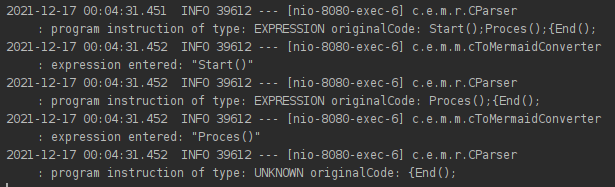
\includegraphics[width=\textwidth]{terminal-log.png}
  \end{subfigure}\hfill
  \caption{Sample log in the terminal from the program run which ended with an error}
\end{figure}
	

\section{Lexer and parser of a C-based language}
	\subsection{Lexer} 
  The Java 11 SE language has a code lexer integrated with the parser and its main task is to recognize instructions handled by applications using regular expressions and to ensure a balanced use of both round and curly brackets in the right order, in accordance with the C programming rules. 

		\break
		
				
\begin{figure}[H]
  \begin{subfigure}{\textwidth}
			\begin{minted}[linenos=true]{java}
ELSE_PATTERN = "\\}else\\{.*";
IF_PATTERN = "if\\(.*";
WHILE_PATTERN = "while\\(.*";
EXPRESSION_PATTERN = "([\\w\\+\\-=\\(\\)\\.,<>/]+?;).*";
END_SCOPE_PATTERN = "\\}.*";
			\end{minted}
  \end{subfigure}\hfill
  \caption{List of recognizable by lexer regular expressions (REGEX patterns)}
\end{figure}
			
	\subsection{Parser} 		
  The code parser is written based on the recursive descent parser used in C/C++ compilers such as: GCC and Clang among others. It consists in recursively calling the function that reads subsequent instructions recognized by the lexer and, depending on the type of these instructions, extracts the argument content (in round brackets) and the content of the internal scope of the instruction (in curly brackets).
						
\begin{figure}[H]
  \begin{subfigure}{\textwidth}
			\begin{minted}[linenos=true]{java}

private void handleIfStatement(){
    String statement = programBuilder.toString();
    String condition = getStringInOuterParenthesis(statement);
    String expressions = getStringInOuterCurly(statement);
    programBuilder.delete(0, condition.length() + 5);
    onIfStatementEnter(condition, expressions);
    parseProgramInstruction();
}
			\end{minted}
  \end{subfigure}\hfill
  \caption{An example function that isolates its argument (condition variable) and the contents of its inner scope (expressions variable) from the $if$ statement, and then passes these values to the so-called observable method (onIfStatementEnter)}
\end{figure}
		
In this case, opening a new scope is possible only in the $if -- else$ and $while$ statements. To support the multiple nesting of those statements, an enumeration representing its statement type with each entry in its scope is pushed onto the stack and later removed from the stack with the scope exit to keep track of the current scope and assure that the correct observable methods are being self-invoked (as in the $Observer$ design pattern). In the case of instructions corresponding to process blocks (any text without the use of special characters, terminated with a semicolon), the observable method informs only about its invocation, while in the case of conditional statements ($if-else$ and $while$), there are methods dedicated to entering and exiting the area of this instruction. The default observable method only displays the basic information about the instruction in the terminal, but this information can be used freely by the version of that class with overwritten definitions of its observable methods. 
						
\begin{figure}[H]
  \begin{subfigure}{\textwidth}
		\begin{minted}[linenos=true]{java}
public void onIfStatementEnter(String condition, String expressions){
  log.info("IF entered : " + condition + " than : " + expressions);
}

public void onIfStatementExit(){
  log.info("IF exited");
}

public void onElseStatementEnter(String expressions){
  log.info("ELSE entered : " + expressions);
}
		\end{minted}
  \end{subfigure}\hfill
  \caption{An example of the default definition of observed methods for a $if/else$ statement}
\end{figure}



\section{Accelerator for building code required by Mermaid}

\begin{figure}[H]
  \begin{subfigure}{\textwidth}
  	\centering
    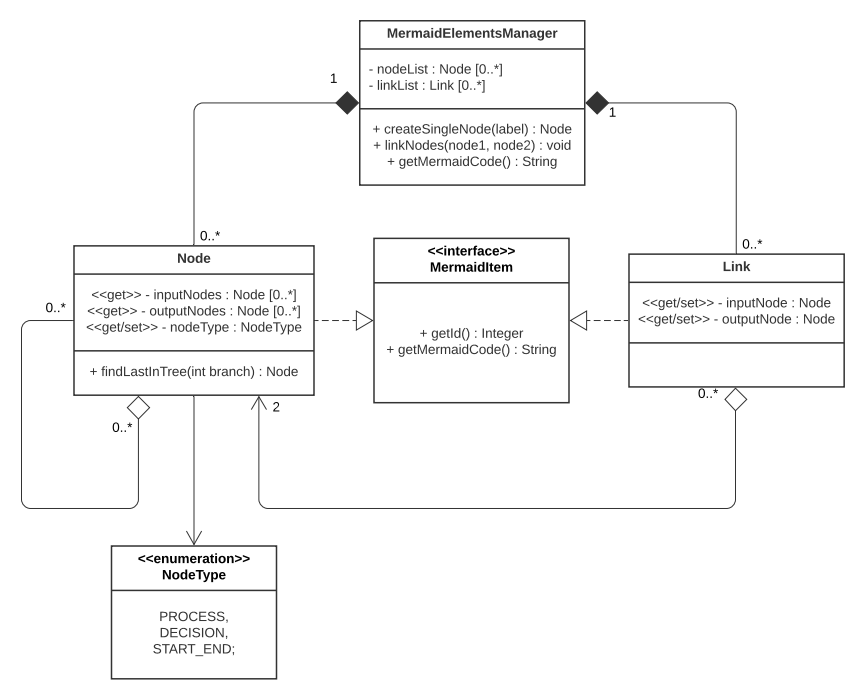
\includegraphics[width=\textwidth]{uml-akcelerator.png}
  \end{subfigure}\hfill
  \caption{UML diagram of classes from which the Mermaid code building accelerator was created}
\end{figure}

To facilitate the creation of flowcharts, an accelerator was created -- a set of classes that allows the programmer to easily create and manage individual elements of flowcharts, and then convert these elements in the program's memory to the target code required by Mermaid. Ultimately, it consists of a list of nodes corresponding to individual blocks and links generated on the basis of relations between these nodes. Using accessors and other public methods detailed in the UML diagram above, the programmer can easily create new nodes, assign the correct type, and connect them together.

\section{Converter from C-based language to Mermaid language}

This converter uses the previously mentioned $Observer$ design pattern. In this case, it overrides the default definitions of the observable methods previously described. Immediately after calling such an overridden method, depending on what action it was assigned to, it performs certain instructions, also using arguments passed by these methods.
	
							
\begin{figure}[H]
  \begin{subfigure}{\textwidth}
		\begin{minted}[linenos=true]{java}
@Override
public void onIfStatementEnter(String condition, String expressions){
    condition = replaceChars(condition);
    condition = wordWrap(condition, 12);
    log.info("IF entered : " + condition + " than : " + expressions);
    manager.setLastNode(fromNode);
    NodeItem scopeNode = manager
            .createDecisionNodeLinkedToLast(condition);
    scopeNodes.push(scopeNode);
    fromNode = scopeNode.getOutputs().get(0);
}

@Override
public void onIfStatementExit(){
    log.info("IF exited");
    manager.createSingleNode("#if_merge");
    manager.linkNodes(scopeNodes.peek().findLastInTree(0), 
            manager.getLastNode());
    manager.linkNodes(scopeNodes.peek().findLastInTree(1), 
            manager.getLastNode());
    scopeNodes.pop();
    fromNode = manager.getLastNode();
}

@Override
public void onElseStatementEnter(String expressions){
    log.info("ELSE entered : " + expressions);
    fromNode = scopeNodes.peek().getOutputs().get(1);
}
		\end{minted}
  \end{subfigure}\hfill
  \caption{Example of overridden observable methods that are being self-invoked as interpretation of the C-based code goes by encountering the $if-else$ statement}
\end{figure}

In the above example, after entering the $if$ (onIfStatementEnter) conditional statement, the condition is subjected to removing all special characters, replacing ``\_'' (underscore) with `` '' (white-space). Then the content of that condition is subjected to a text wrap. Later, after the initially prepared condition content, a node responsible for the decision block is created with the help of the Mermaid code building accelerator. Due to the fact that this node opens a new inner scope, it is added to the stack (scopeNodes) tracking which scope is being executed at the moment. By default, two branches come out of the decision block -- scope opening node is connected (by holding the references in the list of outputs) with two temporary helper nodes (that are removed at the end of code parsing), to the end of the first one (index = 0) the instructions contained in the inner scope are sequentially attached, read recursively according to the parser, while to the last node of the second branch (index = 1), statements are appended when the function corresponding to the $else$ statement is called. After processing all contents of the described conditional statement, another temporary helper node is created that merges both branches when leaving the inner $if-else$ scope (by calling the onIfStatementExit observable method). Finally, the decision node whose scope has just been closed is removed from the stack.